\documentclass[11pt, twocolumn]{article}

\usepackage[spanish]{babel}
\usepackage[none]{hyphenat}
\usepackage[left=1.5cm, right=1.5cm, top = 2cm, bottom=2.5cm]{geometry}
\usepackage{enumitem}
\usepackage{longtable}
\usepackage{multirow, makecell}
\usepackage{listings}
\usepackage{color}
\usepackage{graphicx}
\usepackage{subcaption}
\usepackage{parskip}
\usepackage[hidelinks]{hyperref}
\usepackage{fancyhdr}
\usepackage[export]{adjustbox}

\newcommand{\linejump}{\hfill \break}
\renewcommand{\thefootnote}{\fnsymbol{footnote}}

\definecolor{dkgreen}{rgb}{0,0.6,0}
\definecolor{gray}{rgb}{0.5,0.5,0.5}
\definecolor{mauve}{rgb}{0.58,0,0.82}
\lstset{
  language=Java,
  aboveskip=3mm,
  belowskip=3mm,
  showstringspaces=false,
  columns=flexible,
  basicstyle={\tiny\ttfamily},
  numbers=none,
  numberstyle=\tiny\color{gray},
  keywordstyle=\color{blue},
  commentstyle=\color{dkgreen},
  stringstyle=\color{mauve},
  breaklines=true,
  breakatwhitespace=true,
  tabsize=3
}

\sloppy
\setlength{\parindent}{0cm}
\setlength{\columnsep}{0.5cm}
\decimalpoint
\graphicspath{{img/}}

\hypersetup{colorlinks=true, urlcolor=blue, citecolor=blue}
\urlstyle{same}

\pagestyle{fancyplain}
\fancyhf{}
\fancyhead[L]{\scriptsize 
  Universidad Nacional Autónoma de México \\
  Laboratorio de Programación Orientada a Objetos \\
  M.C. Leonardo Ledesma Dominguez
}
\fancyhead[R]{\thepage}


\begin{document}
  \twocolumn[
    \centering
    Acosta Porcayo Alan Omar, Gutiérrez Grimaldo Alejandro, Medina Villa Samuel

    \linejump

    \LARGE \textbf{Práctica 3. Utilerías y Clases de Uso} \\
    
    \linejump
  ]
      
  \footnotetext{
    \scriptsize 
    Acosta Porcayo Alan Omar Ing. en Computación 320206102 \\
    Gutiérrez Grimaldo Alejandro Ing. en Computación 320282098 \\
    Medina Villa Samuel Ing. en Computación 320249538
  }
        
  \fancyfoot{}

  \section*{Resumen}
  Cuando se programa en un lenguaje de programación, resulta crucial utilizar las bibliotecas incorporadas en ese mismo lenguaje con el fin de ejecutar tareas habituales y repetitivas de manera más eficaz. Para lograrlo, es esencial tener un conocimiento profundo de las bibliotecas disponibles en el lenguaje y aprender a emplearlas de manera apropiada. Asimismo, es posible mejorar la eficiencia del código al utilizar las clases ofrecidas por estas bibliotecas, lo que simplifica el proceso de programación y eleva la calidad del programa

  \section*{Introducción}
  En el mundo de la programación, es crucial aprovechar al máximo las clases preexistentes que pueden satisfacer las necesidades de un programa. Este enfoque se basa en el principio de no ``reinventar la rueda''. Aquí hay más detalles sobre por qué esto es importante:

  \begin{itemize}
    \item \textbf{Ahorro de tiempo}: Reutilizar clases y bibliotecas existentes permite a los desarrolladores ahorrar tiempo valioso. En lugar de escribir código desde cero para cada funcionalidad, pueden aprovechar soluciones probadas y confiables.
    \item \textbf{Mejora de la calidad del software}: Las clases preconstruidas suelen haber pasado por un riguroso proceso de prueba y depuración. Esto significa que son menos propensas a errores y problemas de rendimiento que el código nuevo y no probado.
  \end{itemize}
  
  \subsection*{Arreglos}
  Los arreglos en programación son estructuras de datos que permiten almacenar una colección de elementos del mismo tipo. Aquí hay más información sobre su uso:

  \begin{itemize}
    \item \textbf{Índices numéricos}: Cada elemento en un arreglo se identifica mediante un índice numérico. Los índices comienzan generalmente en 0 (cero) para el primer elemento y aumentan secuencialmente.
    \item \textbf{Declaración y asignación}: Los arreglos se pueden declarar y asignar de varias formas en diferentes lenguajes de programación. En Java, por ejemplo, puedes declarar un arreglo de enteros de la siguiente manera: \textit{int[] numeros = new int[5];}.
    \item \textbf{Acceso a elementos}: Para acceder a un elemento específico en un arreglo, se utiliza su índice. Por ejemplo, \textit{numeros[2]} accedería al tercer elemento en el arreglo (índice 2).
  \end{itemize}

  \subsection*{Argumentos por línea de comandos}
  La capacidad de pasar argumentos por línea de comandos a un programa es útil en muchas situaciones. Aquí hay más información sobre cómo funciona y cuándo es beneficioso:

  \begin{itemize}
    \item \textbf{Versatilidad}: Permite que un programa realice diferentes tareas o se comporte de manera diferente según los argumentos proporcionados al ejecutarlo. Esto lo hace más versátil y reutilizable.
    \item \textbf{Ejemplos comunes}: Algunos ejemplos comunes de uso de argumentos por línea de comandos incluyen proporcionar configuraciones personalizadas, indicar archivos de entrada/salida o activar/desactivar funciones específicas del programa.
  \end{itemize}

  \subsection*{API de Java}
  La API de Java es una vasta biblioteca de clases y métodos proporcionados por los desarrolladores del lenguaje Java. Aquí hay más detalles sobre su importancia:

  \begin{itemize}
    \item \textbf{Amplia funcionalidad}: La API de Java abarca una amplia gama de funcionalidades, desde manipulación de cadenas hasta operaciones matemáticas avanzadas. Esto significa que los desarrolladores pueden acceder a una gran cantidad de herramientas sin tener que escribir todo desde cero.
    \item \textbf{Organización en paquetes}: La API de Java está organizada en paquetes lógicos, lo que facilita la búsqueda y el uso de clases relacionadas. Por ejemplo, las clases de manipulación de archivos se encuentran en el paquete \textit{java.io}.
  \end{itemize}

  \subsection*{Manejo de cadenas}
  El manejo de cadenas es una parte fundamental de la programación, ya que la mayoría de las aplicaciones deben trabajar con texto de alguna forma. Aquí hay más información sobre las operaciones comunes de manejo de cadenas:

  \begin{itemize}
    \item \textbf{Concatenación}: Unir o concatenar cadenas es una operación común. En Java, esto se hace utilizando el operador +. Por ejemplo, ``Hola'' + ``Mundo'' resultaría en ``HolaMundo''.
    \item \textbf{Longitud de cadena}: Puedes determinar la longitud de una cadena utilizando el método \textit{length()}. Esto es útil para saber cuántos caracteres contiene una cadena.
    \item \textbf{Búsqueda de subcadenas}: Puedes buscar subcadenas dentro de una cadena utilizando métodos como \textit{indexOf()} o \textit{contains()}. Esto es útil para buscar palabras clave o patrones en texto.
  \end{itemize}

  \subsection*{\textit{Wrappers}}
  Las clases envoltorio o ``\textit{wrappers}'' en Java son fundamentales para trabajar con tipos primitivos como enteros, flotantes, etc. Aquí hay más información sobre su utilidad:

  \begin{itemize}
    \item \textbf{Conversión de tipos}: Los wrappers permiten convertir tipos primitivos en objetos y viceversa. Por ejemplo, puedes convertir un \textit{int} en un \textit{Integer} utilizando \textit{wrappers}.
    \item \textbf{Usos comunes}: Los \textit{wrappers} son especialmente útiles cuando se trabaja con colecciones de objetos, ya que las colecciones generalmente requieren objetos en lugar de tipos primitivos.
  \end{itemize}

  \subsection*{Colecciones}
  Las colecciones en Java son estructuras de datos que permiten almacenar y manipular grupos de objetos. Aquí hay más información sobre las colecciones y sus tipos comunes: 
  
  \begin{itemize}
    \item \textbf{Dinámicas}: A diferencia de los arreglos estáticos, las colecciones pueden cambiar de tamaño dinámicamente a medida que se agregan o eliminan elementos.
    \item \textbf{Tipos comunes}: Algunos tipos comunes de colecciones en Java incluyen listas (por ejemplo, \textit{ArrayList}), conjuntos (por ejemplo, \textit{HashSet}) y mapas (por ejemplo, \textit{HashMap}).
    \item \textbf{Operaciones básicas}: Las operaciones comunes en colecciones incluyen agregar elementos, eliminar elementos, buscar elementos y recorrer la colección para realizar diversas operaciones.
  \end{itemize}

  \subsection*{Clases de utilerías}
  Java proporciona una serie de clases de utilería que simplifican tareas comunes, como cálculos matemáticos y manipulación de fechas. Algunas de las clases más útiles son:

  \begin{itemize}
    \item \textbf{\textit{Math}}: La clase \textit{Math} proporciona métodos para realizar operaciones matemáticas avanzadas, como exponenciación, raíz cuadrada y funciones trigonométricas.
    \item \textbf{\textit{Date} y \textit{Calendar}}: Estas clases permiten trabajar con fechas y horas, realizar cálculos de tiempo y dar formato a las fechas según las necesidades del programa.
  \end{itemize}

  \section*{Objetivos}
  \begin{itemize}
    \item Utilizar bibliotecas estándar como punto de partida para aprender y comprender conceptos y técnicas de programación antes de explorar soluciones personalizadas.
    \item Utilizar bibliotecas para incorporar funcionalidades probadas y confiables, mejorando así la calidad del código.
    \item Aprender a adaptar y personalizar las bibliotecas para satisfacer necesidades específicas sin tener que crear soluciones desde cero.
  \end{itemize}

  \section*{Metodología} 
  \subsection*{Ejercicio realizado por el profesor}
  
  \textbf{Código}
  \begin{lstlisting}
import java.util.Hashtable;
import java.time.LocalDate;
import java.util.Enumeration;
import java.util.ArrayList;
import java.time.LocalDate;

public class pract3 {
  public static void main(String[] args) {
    int[] nums = new int[10];
    for(int i = 0; i < nums.length; i++) {
      nums[i] = i * 2;
    }

    //foreeach
    for(int k: nums) {
      System.out.println(k);
    }

    int[][] m = new int[5][5];
    for(int i = 0; i < m.length; i++) {
      for(int j = 0; j < m[0].length; j++) {
        if(i == j) {
          m[i][j] = 1;
        }
      }
    }

    for(int i = 0; i < m.length; i++) {
      for(int j = 0; j < m[0].length; j++) {
        System.out.print(m[i][j] + " ");
      }
      System.out.println();
    }

    String a = args[0];
    int n = Integer.parseInt(args[1]); // moldeaado o casting

    System.out.println("El GOAT es: " + a + " : " + n);

    String s = "Samuel el reprobado de POO GRUPO 3";

    s = s.toUpperCase();
    System.out.println(s);

    StringBuilder sb = new StringBuilder(s);
    sb.append(" por irle a MESSI");
    System.out.println(sb);

    Hashtable<String,String> atlas = new Hashtable<String,String>();

    atlas.put("Mexico", "CDMX");
    atlas.put("Rusia ", "Moscu");
    atlas.put("Etiopia", "Addis Abeba");
    atlas.put("Marruecos", "Rabat");
    atlas.put("Sudafrica", "Pretoria");

    String pais;
    String capital;

    Enumeration<String> claves = atlas.keys();

    while(claves.hasMoreElements()) {
      pais = claves.nextElement();
      capital = atlas.get(pais);

      System.out.println("Pais:  " + pais + " su capital es " + capital);
    }

    ArrayList<String> programastv = new ArrayList<String>();

    programastv.add("Tortugas Ninja");
    programastv.add("Hey Arnold!");
    programastv.add("Los chicos del barrio");
    programastv.add("Los cuentos de la calle broca");
    programastv.add("Zobomafuu y los hermanos Krat");
    programastv.add("Power Rangers");

    programastv.remove(0);

    for(String pr: programastv) {
      System.out.println(pr);
    }

    LocalDate hoy = LocalDate.now();
    System.out.println(hoy);
  }
}
  \end{lstlisting} 

  \section*{Resultados}
  \subsection*{Problema 1}
  Elaboré el modelo de encriptación antiguo llamado \textit{Scytale}. Ubicado en: \url{https://edabit.com/challenge/KXs93N4RX6jNSsgCr}. 
  
  \textbf{Utilice el manejo de cadenas y arreglos matriciales}.

  \begin{figure}[ht]
    
\includegraphics[width=0.5\columnwidth, center]{Scytale.png}
  \end{figure}

  \textbf{Explicación} \\
  El programa funciona a partir de un mensaje y un entero positivo ingresados por el usuario. El mensaje y el entero se mandan como parámetros a la función \textit{cipher}, en la cual primero se obtiene la longitud del mensaje y se crea una copia del mensaje instanciando la clase \textit{StringBuilder}. Para cifrar el mensaje se necesita una matriz utilizando el valor de n como las filas y dividiendo la longitud del mensaje entre n (si esta división tiene residuo, se le suma 1 y a la copia del mensaje se le agregan espacios en blanco). A la matriz se le asignan los caracteres de la copia del mensaje fila por fila y a otra cadena se le agregan los caracteres de la matriz columna por columna. Por último se retorna el mensaje cifrado y se imprime.

  \textbf{Código}
  \begin{lstlisting}
import java.util.Scanner;

public class Problema1 {
  static StringBuilder cipher(String m, int n) {
    int mLen = m.length();
    int cols;
    StringBuilder sb = new StringBuilder(m);

    if (mLen % n != 0) {
      cols = (mLen / n) + 1;
      for(int i = 0; i < (n * cols) - mLen; i ++)
        sb.append(' ');
    } else 
      cols = mLen / n;
    
    char[][] matrix = new char[n][cols];
    for(int i = 0; i < matrix.length; i ++) {
      for(int j = 0; j < matrix[0].length; j ++)
        matrix[i][j] = sb.charAt((i * cols) + j);
    }
    
    StringBuilder cipher = new StringBuilder();
    for(int i = 0; i < matrix[0].length; i ++) {
      for(int j = 0; j < matrix.length; j ++)
        cipher.append(matrix[j][i]);
    }

    return cipher;
  }

  public static void main(String[] args) {
    Scanner sc = new Scanner(System.in);
    String mensaje;
    int n;

    System.out.print("Mensaje: ");
    mensaje = sc.nextLine();
    do {
      System.out.print("n: ");
      n = sc.nextInt();
      if (n <= 0)
        System.out.println("n debe ser positivo\n");
    } while(n <= 0);

    System.out.println("\n" + cipher(mensaje, n));

    sc.close();
  }
}    
  \end{lstlisting}

  \textbf{Terminal}
  \begin{figure}[ht]
    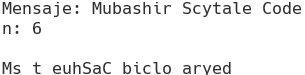
\includegraphics[width=0.6\columnwidth, center]{P1.png}
  \end{figure}


  \subsection*{Problema 2}
  Simule un sistema de inscripciones para los alumnos de una universidad, el alumno podrá:

  \begin{enumerate}[label=\alph*.]
    \item Inscribirse a una materia.
    \item Darse de baja en una materia.
    \item Ver el historial de su inscripción en cualquier momento.
    \item Finalizar inscripción (mostrar un resumen de sus materias)
  \end{enumerate}

  Considere las siguientes clases de tipo publicas alumno (nombre, apellido materno, apellido paterno, número de cuenta, edad y sexo), materia o asignatura (clave de la materia, nombre de la materia, créditos y cupo) y el sistema de inscripción donde estará el método \textit{Main}.

  El (los) alumno(s) tienen que darse de alta en el sistema de inscripción primeramente para luego realizar su inscripción cuando un alumno termine su inscripción. El sistema seguirá abierto para una nueva alta de alumno. Si la materia ya no tiene cupo no permite realizar la inscripción y manda mensaje de CUPO LLENO.

  Al final el programa se deberá mostrar el listado de cada alumno y su inscripción, así como cada materia con su cupo final.

  \textbf{Utilice clases públicas y atributos de tipo privado, \textit{getters and setters, Hashtable} para las materias y \textit{Arraylist} para la inscripción de alumnos, o cualquier otro tipo de colección que considere mejor.}.

  \textbf{Explicación} \\
  

  \textbf{Código}
  % \begin{lstlisting}

  % \end{lstlisting}
  
  \textbf{Terminal}
  % \begin{figure}[ht]
  %   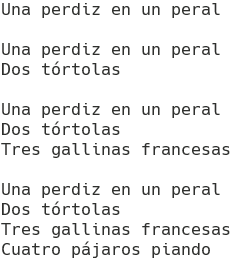
\includegraphics[width=0.38\columnwidth, center]{P2A.png}
  % \end{figure}

  \subsection*{Problema 3}
  Programe el juego de la tortuga y la liebre.

  \begin{figure}[ht]
    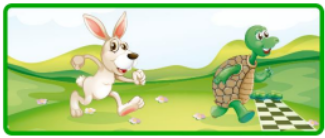
\includegraphics[width=0.6\columnwidth, center]{TortugaLiebre.png}
  \end{figure}
  
  En consola de debe de mostrar siempre la pista de 100 unidades en una matriz de 10$\times$10 de esta manera:

  \begin{figure}[ht]
    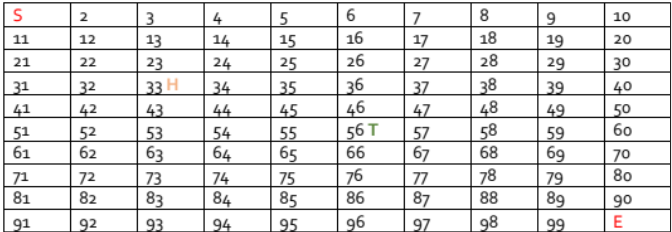
\includegraphics[width=\columnwidth, center]{Pista.png}
  \end{figure}

  \textbf{Donde S es \textit{Start}, E es \textit{End}, H es \textit{Hare} (Liebre) y T es \textit{Turtle}}.

  Se lanzará un dado por cada jugador y siempre arrancará la Tortuga. Si la Tortuga o la Liebre llegan a los siguientes números:

  \begin{itemize}
    \item 7, 14, 33, 77 y 89 se obtiene una segunda tirada.
    \item 6, 23, 42, 56, 82, 90 el jugador se regresa 5 casillas para atrás.
    \item 36 y 65 son números especiales ambos van al 71 y al 84.
    \item El 10 regresa al inicio del juego y 66 regresa al 40.
  \end{itemize}

  \textbf{Utilice arreglos matriciales y un numero aleatorio para simular el dado}.

  \textbf{Explicación} \\
  El programa funciona a partir de 4 métodos y una variable de clase que representa la pista de $10\times 10$. El método \textit{inicio} le asigna a las casillas el número de la posición o un carácter si es el inicio o el final de la pista. El método \textit{pista} imprime la matriz usando dos ciclos \textit{for}. El método \textit{jugada} toma como parámetro la posición actual del jugador en turno y le suma un número aleatorio entre 1 y 6 simulando un dado. Las estructuras \textit{if} comprueban si se cayo en una casilla especial para realizar una operación extra.

  Por último, el método \textit{main} inicializa la pista y dentro de un ciclo \textit{while} sucede cada turno. Los turnos impares son de la tortuga y los pares de la liebre. En cada turno se llama al método \textit{jugada} y se obtiene un nueva posición. Luego se elimina el carácter que representa al jugador en la casilla en la que estaba antes de la tirada de dado, para colocar el carácter en la nueva posición. El juego termina hasta que algún jugador llegue a la casilla 100. 

  \textbf{Código}
  \begin{lstlisting}
import java.util.Random;

public class Problema3 {
  static StringBuilder[][] p = new StringBuilder[10][10];

  static void inicio() {
    int k = 2;

    p[0][0] = new StringBuilder("S");
    p[9][9] = new StringBuilder("E");

    for(int i = 0; i < p.length; i ++) {
      for(int j = 0; j < p[0].length; j ++){
        if((i == 0 && j == 0) || (i == 9 && j == 9))
          continue;
        else {
          p[i][j] = new StringBuilder(Integer.toString(k));
          k ++;
        }
      }
    }

    p[0][0].append("HT");
  }

  static void pista() {
    for(int i = 0; i < p.length; i ++) {
      for(int j = 0; j < p[0].length; j ++)
        System.out.print(p[i][j] + "\t");
      System.out.println();
    }
  }

  static int jugada(int nPos) {
    Random rand = new Random();
    int d, n = nPos;

    d = rand.nextInt(6) + 1;
    n += d;

    if (n > 100)
      n = 100;

    System.out.println("Dado: " + d);
    System.out.println("Avanza de " + nPos +" a " + n);
    
    if(n == 7 || n == 14 || n == 33 || n == 77 || n == 89) {
      System.out.println("Casilla Especial!\tTira de nuevo");
      n = jugada(n);
    } else if(n == 6 || n == 23 || n == 42 || n == 56 || n == 82 || n == 90) {
      System.out.println("Trampa\tRetrocede de " + n + " a " + (n - 5));
      n -= 5;
    } else if(n == 36) {
      System.out.println("Casilla Especial!\tAvanza de " + n + " a 71");
      n = 71;
    } else if(n == 65) {
      System.out.println("Casilla Especial!\ttAvanza de " + n + " a 84");
      n = 84;
    } else if(n == 10) {
      System.out.println("Trampa\tRegresa al inicio");
      n = 1;
    } else if(n == 66) {
      System.out.println("Trampa\tRegresa de " + n + " a 40");
      n = 40;
    }

    return n;
  }

  public static void main(String[] args) {
    int posIH = 0, posJH = 0, posIT = 0, posJT = 0, nH = 1, nT = 1, turno = 0;

    inicio();        

    System.out.println("Pista inicial");
    pista();

    while(true) {
      turno ++;

      System.out.print("\nTurno " + turno);	
      if(turno % 2 != 0){
        System.out.println(". Tira la Tortuga\n");
        
        nT = jugada(nT);

        if(p[posIT][posJT].charAt(p[posIT][posJT].length() - 1) == 'T')
          p[posIT][posJT].deleteCharAt(p[posIT][posJT].length() - 1);
        else
          p[posIT][posJT].deleteCharAt(p[posIT][posJT].length() - 2);
        
        if(nT == 0) {
          posIT = 0;
          posJT = 0;
        } else {
          posIT = (nT - 1) / 10;
          posJT = (nT - 1) % 10;
        }

        p[posIT][posJT].append("T");
      } else {
        System.out.println(". Tira la Liebre\n");
        
        nH = jugada(nH);

        if(p[posIH][posJH].charAt(p[posIH][posJH].length() - 1) == 'H')
          p[posIH][posJH].deleteCharAt(p[posIH][posJH].length() - 1);
        else
          p[posIH][posJH].deleteCharAt(p[posIH][posJH].length() - 2);

        if(nH == 0) {
          posIH = 0;
          posJH = 0;
        } else {
          posIH = (nH - 1) / 10;
          posJH = (nH - 1) % 10;
        }

        p[posIH][posJH].append("H");
      }
      
      pista();
      
      if(nH == 100 || nT == 100)
        break;

      System.out.println("Fin del turno\n");
    }

    System.out.println("\nGanador: " + (turno % 2 != 0 ? "Tortuga!" : "Liebre!"));
    System.out.println("Fin del juego");
  }
}    
  \end{lstlisting}

  \textbf{Terminal}
  \begin{figure}[ht]
    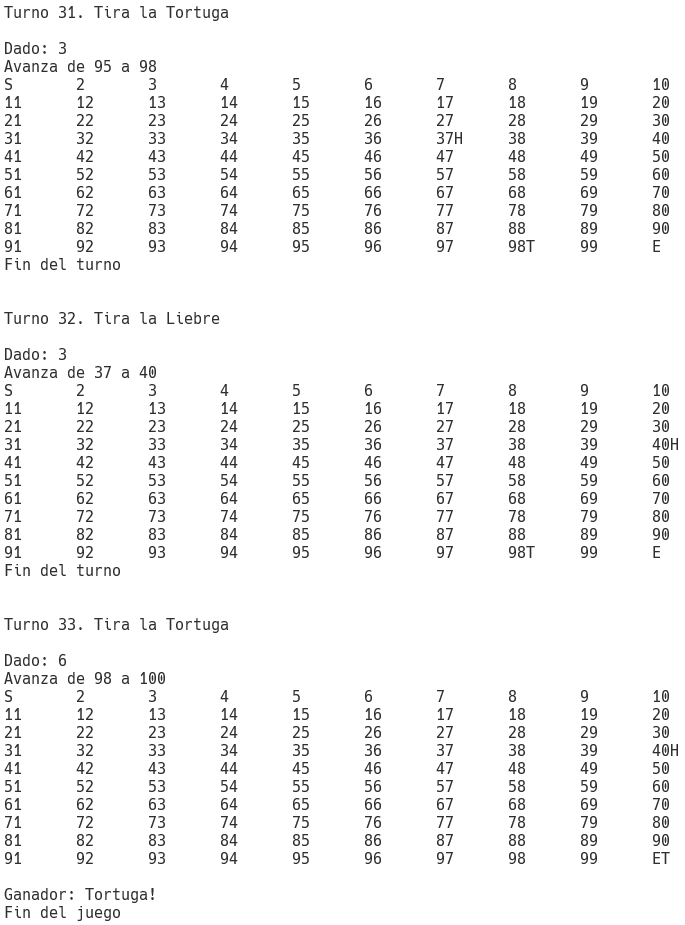
\includegraphics[width=\columnwidth, center]{P3.png}
  \end{figure}

  \subsection*{Problema 4}
  Cree 4 conjuntos $A$, $B$, $C$, $D$, llene los conjuntos de manera aleatoria de tamaño 10, 20, 30 y 40 respectivamente de números aleatorios entre 0 y 200. Encuentre los siguientes valores:

  \begin{enumerate}[label=\alph*.]
    \item $A \cap B \cap C \cap D$
    \item $(A \cap B) \cup (C \cap D)$
    \item Calcule el $U = A \cup B \cup C \cup D$ sin repetición de elementos.
    \item $B - U = B^C$ 
  \end{enumerate}

  \textbf{Utilice Sets y sus operaciones}.

  \textbf{Explicación} \\
  

  \textbf{Código}
  % \begin{lstlisting}

  % \end{lstlisting}

  \textbf{Terminal}
  % \begin{figure}[ht]
  %   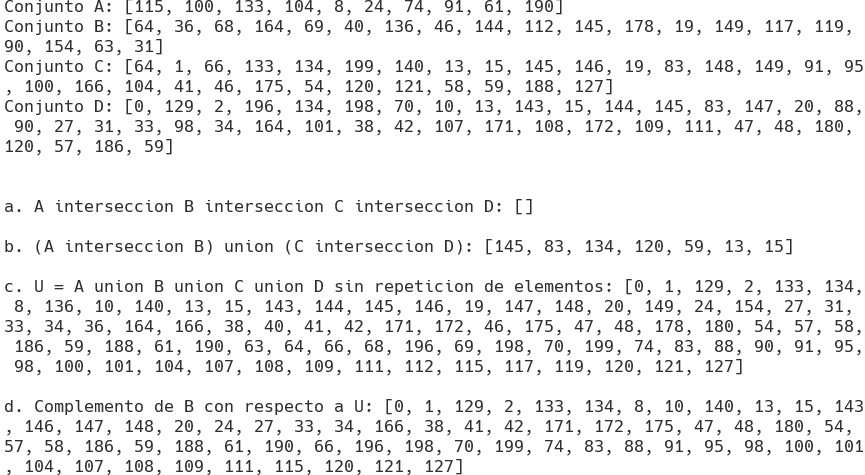
\includegraphics[width=0.15\columnwidth, center]{P4.png}
  % \end{figure}

  \subsection*{Problema 5}
  Construya un árbol genealógico \textbf{sencillo} de cualquier panteón mitológico (griego, romano, nórdico, etc) seleccione cualquier tipo de estructura tipo Tree que java ofrece. De manera tal que una estructura de tipo Tree es una persona y sobre el estarán sus hij@s.

  \begin{figure}[ht]
    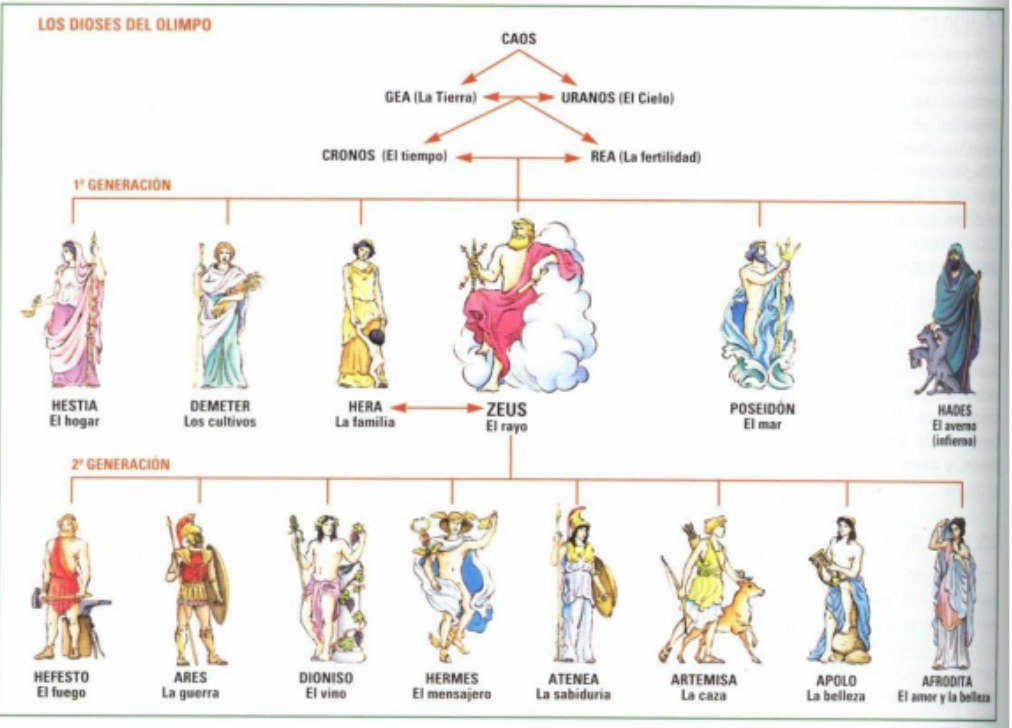
\includegraphics[width=\columnwidth, center]{Arbol.png}
  \end{figure}
  
  Ejemplo:

  Cronos $\rightarrow$ Zeus, Poseidón, Hades \\
  Zeus $\rightarrow$ Hermes, Atenea, Artemisa, Apolo, Afrodita

  Y podemos buscar sus descendientes, borrar, o agregar. Y buscar sus antecesores.

  \textbf{Explicación} \\
  

  \textbf{Código}
  % \begin{lstlisting}

  % \end{lstlisting}

  \textbf{Terminal}
  % \begin{figure}[ht]
  %   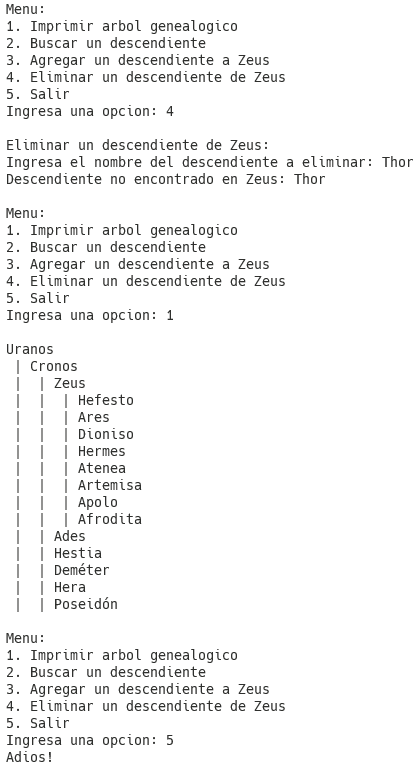
\includegraphics[width=0.75\columnwidth, center]{P5.png}
  % \end{figure}

  \section*{Conclusiones}
  La incorporación de bibliotecas en la programación se convierte en un recurso crucial para potenciar la eficacia, la calidad y la cooperación en el proceso de desarrollo de software. Estas bibliotecas ofrecen soluciones previamente diseñadas para tareas comunes, lo que conlleva ahorro de tiempo y minimiza la probabilidad de cometer errores. Asimismo, fomentan la capacidad de reutilizar código. En última instancia, adquirir destrezas en la utilización de bibliotecas se convierte en una habilidad esencial y contribuye al logro de éxitos en el ámbito de la programación.

  \section*{Referencias}
  \small
  Solano, J. (2017, 20 enero). \textit{Manual de prácticas de Programación Orientada a Objetos}. Laboratorio de Computación Salas A y B. \url{http://lcp02.fi-b.unam.mx/} \\

  Deep Xavier. \textit{Spartans Cipher}. Edabit. \url{https://edabit.com/challenge/KXs93N4RX6jNSsgCr}
\end{document}